\documentclass{InsightArticle}

\usepackage[dvips]{graphicx}
\usepackage{amssymb}
\usepackage{caption}
\usepackage{subcaption}
\usepackage{wrapfig}
\usepackage{listing}					%Used for list of listings
\usepackage{listings}					%List program code source
\usepackage{amsfonts}					%Maths fonts
\graphicspath{{Figures/}}                %List folders to figures here
\usepackage{color}

\usepackage[dvips,
bookmarks,
bookmarksopen,
backref,
colorlinks,linkcolor={blue},citecolor={blue},urlcolor={blue},
]{hyperref}

%%%%%%%%%%%%%%%%%%%%%%%%%%%%%%%%%%%%%%%%%%%%%%%%%%%%%%%%%%%%%%%%%%
% Customizations

%Set default font
%\renewcommand{\familydefault}{\rmdefault}	%Roman
\renewcommand{\familydefault}{\sfdefault}	%Sans serif
%\renewcommand{\familydefault}{\ttdefault}	%Typewriter

%Define some colors
\definecolor{colorgridback}{rgb}{0.975,0.975,0.975}
\definecolor{colorgridlines}{gray}{0.125}
\definecolor{colorbarsub}{rgb}{0.85,0.2,0.2}
\definecolor{darkgreen}{rgb}{0.0,0.2,0.0}
\definecolor{darkgreenwlink}{rgb}{0.0,0.2,0.1}
\definecolor{darkred}{rgb}{0.25,0.0,0.0}
\definecolor{darkblue}{rgb}{0.0,0.0,0.25}
\definecolor{listcomment}{rgb}{0.0,0.5,0.0}
\definecolor{listkeyword}{rgb}{0.0,0.0,0.5}
\definecolor{listbackground}{gray}{0.965}

% for code formatting
% Setup source code listings 
\lstset{frame = tb,
        framerule = 0.5pt,
        float,
        fontadjust,
        backgroundcolor={\color{listbackground}},
        basicstyle = {\ttfamily\footnotesize},
        keywordstyle = {\ttfamily\color{listkeyword}\textbf},
        identifierstyle = {\ttfamily},
        commentstyle = {\ttfamily\color{listcomment}\textit},
        stringstyle = {\ttfamily},
        showstringspaces = false,
        showtabs = false,
        frame=none,
        %captionpos = b,
        tabsize = 2
}
\def\code#1{\small\textcolor{darkgreen}{\texttt{#1}}}
\def\cmdargs#1{\small\textcolor{darkred}{\texttt{#1}}}
\def\vtk#1{\href{www.vtk.org/doc/nightly/html/class#1.html}{\small\textcolor{darkblue}{\texttt{#1}}}}
%%%%%%%%%%%%%%%%%%%%%%%%%%%%%%%%%%%%%%%%%%%%%%%%%%%%%%%%%%%%%%%%%%


\title{Geodesic Computations on Surfaces}
\newcommand{\IJhandlerIDnumber}{3415}

% 
% NOTE: This is the last number of the "handle" URL that 
% The Insight Journal assigns to your paper as part of the
% submission process. Please replace the number "1338" with
% the actual handle number that you get assigned.
%
%\newcommand{\IJhandlerIDnumber}{9999}

% Increment the release number whenever significant changes are made.
% The author and/or editor can define 'significant' however they like.
%\release{1.0}

% At minimum, give your name and an email address.  You can include a
% snail-mail address if you like.
\author{Karthik Krishnan}
%\authoraddress{karthik.krishnan@kitware.com}

\begin{document}

%
% Add hyperlink to the web location and license of the paper.
% The argument of this command is the handler identifier given
% by the Insight Journal to this paper.
% 
\IJhandlefooter{\IJhandlerIDnumber}


\ifpdf
\else
   %
   % Commands for including Graphics when using latex
   % 
   \DeclareGraphicsExtensions{.eps,.jpg,.gif,.tiff,.bmp,.png}
   \DeclareGraphicsRule{.jpg}{eps}{.jpg.bb}{`convert #1 eps:-}
   \DeclareGraphicsRule{.gif}{eps}{.gif.bb}{`convert #1 eps:-}
   \DeclareGraphicsRule{.tiff}{eps}{.tiff.bb}{`convert #1 eps:-}
   \DeclareGraphicsRule{.bmp}{eps}{.bmp.bb}{`convert #1 eps:-}
   \DeclareGraphicsRule{.png}{eps}{.png.bb}{`convert #1 eps:-}
\fi


\maketitle


\ifhtml
\chapter*{Front Matter\label{front}}
\fi


% The abstract should be a paragraph or two long, and describe the
% scope of the document.
\begin{abstract}
\noindent

The computation of geodesic distances on a triangle mesh has many applications in geometry processing. The fast marching method provides an approximation of the true geodesic distance field. We provide VTK classes to compute geodesics on triangulated surface meshes. This includes classes for computing the geodesic distance field from a set of seeds and to compute the geodesic curve between source and destination point(s) by back-tracking along the gradient of the distance field. The fast marching toolkit~\cite{Peyre06} is internally used. A variety of options are exposed to guide front propagation including the ability to specify propagation weights, constrain to a region, specify exclusion regions, and distance based termination criteria. Interpolators that plug into a contour widget, are provided to enable interactive tracing of paths on meshes.
%
\end{abstract}

\IJhandlenote{\IJhandlerIDnumber}

\tableofcontents

%
\section{Theoretical background}
The computation of geodesic distances on a triangle mesh has many applications in geometry processing.
The fast marching method provides an approximation of the true geodesic distance field.
This geodesic distance to a collection of points satisfies a non-linear differential equation, namely the Eikonal equation. The viscosity solution $\phi(x,y)$ of the Eikonal equation given by

\begin{equation}
  \left|\left|\nabla \phi \right|\right| = F
\label{eq:Eikonal}
\end{equation}

is a weighted distance map from a set of initial (seed) points, where the value of $\phi$ is provided, or typically assumed to be 0. The weights are given by the function $F(x,y)$ which is a scalar positive function. In the special case where the function $F(x,y)$ is a constant, $\phi$ can be interpreted as the distance function to the set of seeds. The level set curve, $C_t$, defined as points on the front of the function $\phi$ at time $t$ propagates following the evolution equation

\begin{equation}
  \frac{\delta}{\delta t}C_t(x,y) = \frac{n_{xy}}{P(x,y)}
\label{eq:LevelSet}
\end{equation}

where $n_{xy}$ is the exterior unit normal vector to the curve at the point $(x,y)$. The function $F(x,y) = 1/P(x,y)$ is the propagation speed of the front, $C_t$.

Efficient numerical solutions were introduced by Sethian~\cite{Sethian98} and adapted by Kimmel~\cite{Kimmel98} on triangulated manifolds:

\begin{equation}
  \left|\left|\nabla_M \phi \right|\right| = F
\label{eq:EikonalOnManifolds}
\end{equation}

where $\nabla_M \phi$ is the gradient on the manifold, M. For further details, the reader is referred to ~\cite{Sethian98,Kimmel98,Peyre06}.

A geodesic path between two points may be computed from the distance map, $\phi$ to one of the points, by performing a gradient descent on the function $\phi$.

\section{VTK Interface}

The VTK classes utilize the fast marching library ~\cite{PeyreCode} from Gabriel Peyre provided under a BSD license. The VTK classes act as a wrapper around the library providing the bridge between datastructures and callbacks in both libraries. This section serves as a user guide for the VTK classes. 

\subsection{Geodesic distances - vtkFastMarchingGeodesicDistance}
In the simplest use case, \code{vtkFastMarchingGeodesicDistance} takes in a \vtk{vtkPolyData} reprsentative of a triangle mesh and produces as output the same polydata with point attributes containing the distance field from a seed, or set of seeds.
It derives from an abstract base class \code{vtkPolyDataGeodesicDistance}, which inturn derives from \vtk{vtkPolyDataAlgorithm}.

\subsubsection{Propagation weights}
By default the filter assumes a constant propagation speed. However propagation weights may be explicitly specified by the user using \code{SetPropagationWeights}. This takes as argument, a float/double array, with as many entries as the number of vertices on the mesh. For instance the the mesh curvature may be used to propagate quickly in areas of low curvature and slowly in areas of high curvature. Note that the propagation weights specified must be strictly positive for fast marching to be numerically stable.

\subsubsection{Exclusion Regions}
Optionally, exclusion regions may be specified via \code{SetExclusionPointIds(vtkIdList*)}. Vertices with ids that are in the exclusion list are ommitted from inclusion in the fast marching front. This can be used to prevent bleeding into certain regions. If the specified point ids form a closed, fully connected loop, this effectively serves as an exclusion region boundary. Conversely, it can be used to confine fast marching to a specific region.

\subsubsection{Termination Criteria}
The fast marching may be prematurely terminated via any of the following optional
stopping criteria. These are:

\begin{itemize}
\item \textit{Distance stop criterion}: Propagation stops if any portion of the
front has traversed more than the specified distance from the seed(s).
See \code{SetDistanceStopCriterion(float)}. 
\item \textit{Destination vertex stop criterion}: Propagation stops if any
point in the front arrives at the user supplied destination vertex id(s).
See \code{SetDestinationVertexStopCriterion(vtkIdList*)}. This strategy is used when computing the geodesic
path interactively using the contour line interpolator (described later).
\item \textit{Boundaries}: If a boundary is specified via \code{SetExclusionPointIds} forming a closed boundary around the seeds, propagation terminates when all vertices contained within the boundary have been visited.
\end{itemize}

\subsubsection{Events}
The filter reports IterationEvents. It does not report progress events,
since its not possible to determine when the front might terminate.

\subsubsection{Miscellaneous}
Other options include (a) querying the maximum distance marched by the front 
(b) setting the outside value (for vertices that may not been visited) (c) specifying the distance field name and the ability to turn off its generation (for instance computing the path need not allocate storage for a field on each vertex)


\subsection{Tracing geodesic paths}

\begin{figure}
  \centering
  \begin{subfigure}[b]{0.5\textwidth}
    \centering
    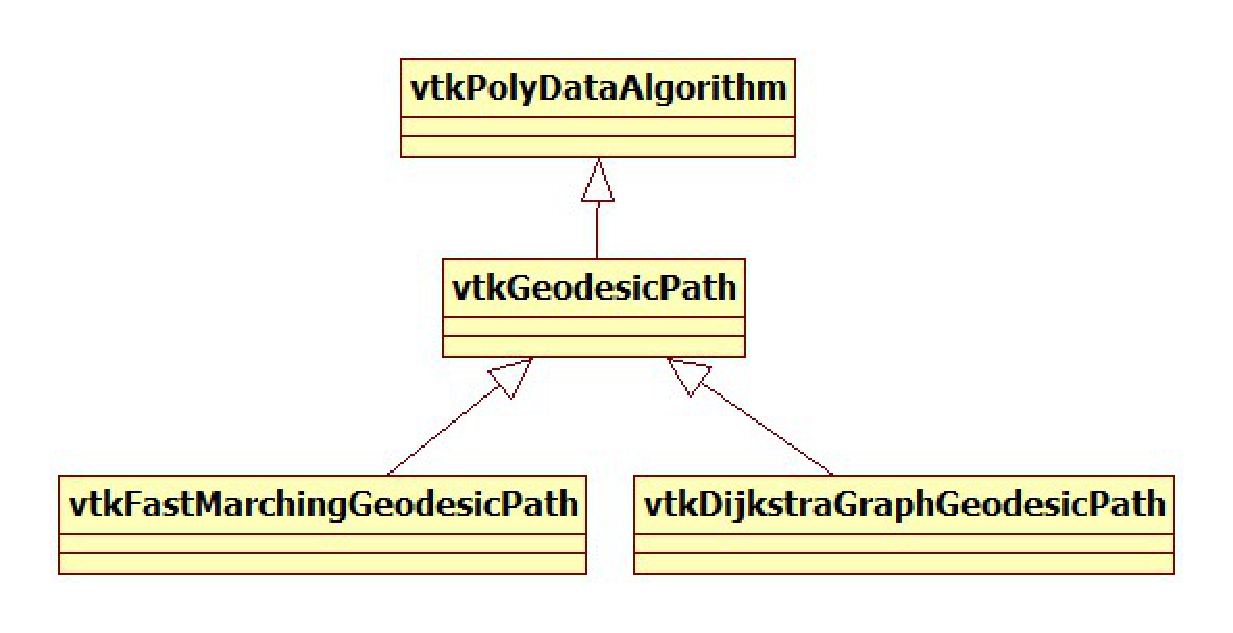
\includegraphics[width=\textwidth]{GeodesicPathUML}
    \caption{Geodesic paths may be computed from a single source to destination vertices using the Dijkstra algorithm or by gradient backtracking of the distance field generated by fast marching.}
    \label{fig:GeodesicPathUML}
  \end{subfigure}%
  ~ %add desired spacing between images, e. g. ~, \quad, \qquad etc.
    %(or a blank line to force the subfigure onto a new line)
  \begin{subfigure}[b]{0.5\textwidth}
    \centering
    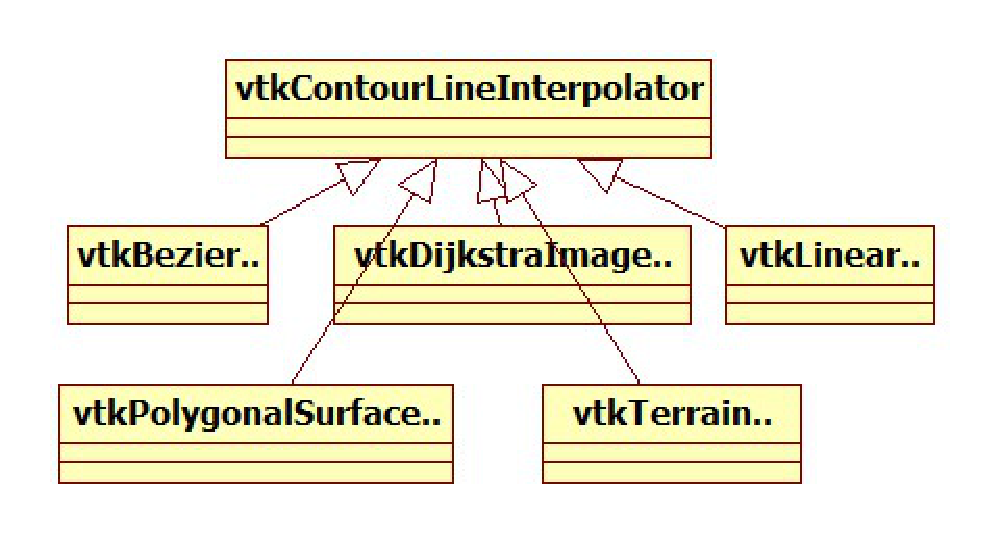
\includegraphics[width=\textwidth]{ContourLineInterpolatorsUML}
    \caption{The vtkPolygonalSurfaceContourLineInterpolator2 is an interpolator that can be used by a contour widget to trace paths on surfaces. These can use either instance of the geodesic path shown on the left.}
    \label{fig:ContourLineInterpolatorUML}
  \end{subfigure}
\caption{ }
\label{fig:GeodesicUMLs}
\end{figure}

The class \code{vtkFastMarchingGeodesicPath} (fig.~\ref{fig:GeodesicUMLs}(a)) computes geodesic paths on triangle meshes. It takes as input a triangle mesh, a set of destination vertex ids and a source vertex id. The geodesic path is generated by traversing along the gradient of the distance field to arrive at a destination vertex.


Internally an instance of \code{vtkFastMarchingGeodesicDistance} is used, and the same options that guide/control front propagation can be used when computing the path.
The distance field computation is performed such that it terminates when the target seed has been reached so that it is localized and fast enough for interactive tracing. The path extraction alone has an $O(N)$ complexity, where N is the number of vertices in the path. The front propagation takes $O(m log m)$ where $m$ is the number of vertices contained in a circular patch of radius spanning the distance between the source and destination vertex. When the source and destination points are no more than a few thousand vertices apart the path extraction is done in milliseconds and is suitable for real time tracing and editing of paths on meshes.

Paths may be generated so that they traverse between mesh vertices (linear interpolation) or may be constrained on mesh vertices. The method \code{SetInterpolationOrder} allows one set the path interpolation order. A zeroth
order path passes through vertices of the mesh. A first order path passes
in between vertices (linear interpolation is performed on the triangle edges).
Each point in the first order path is guarenteed to lie on a triangle edge.

A maximum path length may optionally be specified, in which case, the gradient based
back-tracking may stop prematurely (once the specified length is exceeded).

The point ids of the vertices on the mesh (in case of zeroth order interpolation) or closest
vertices on the mesh (in case of first order interpolation) that connect the source to the destination
point may be queried. This can be used for interactive surface clipping.

\begin{figure}
  \centering
  \begin{subfigure}[b]{0.5\textwidth}
    \centering
    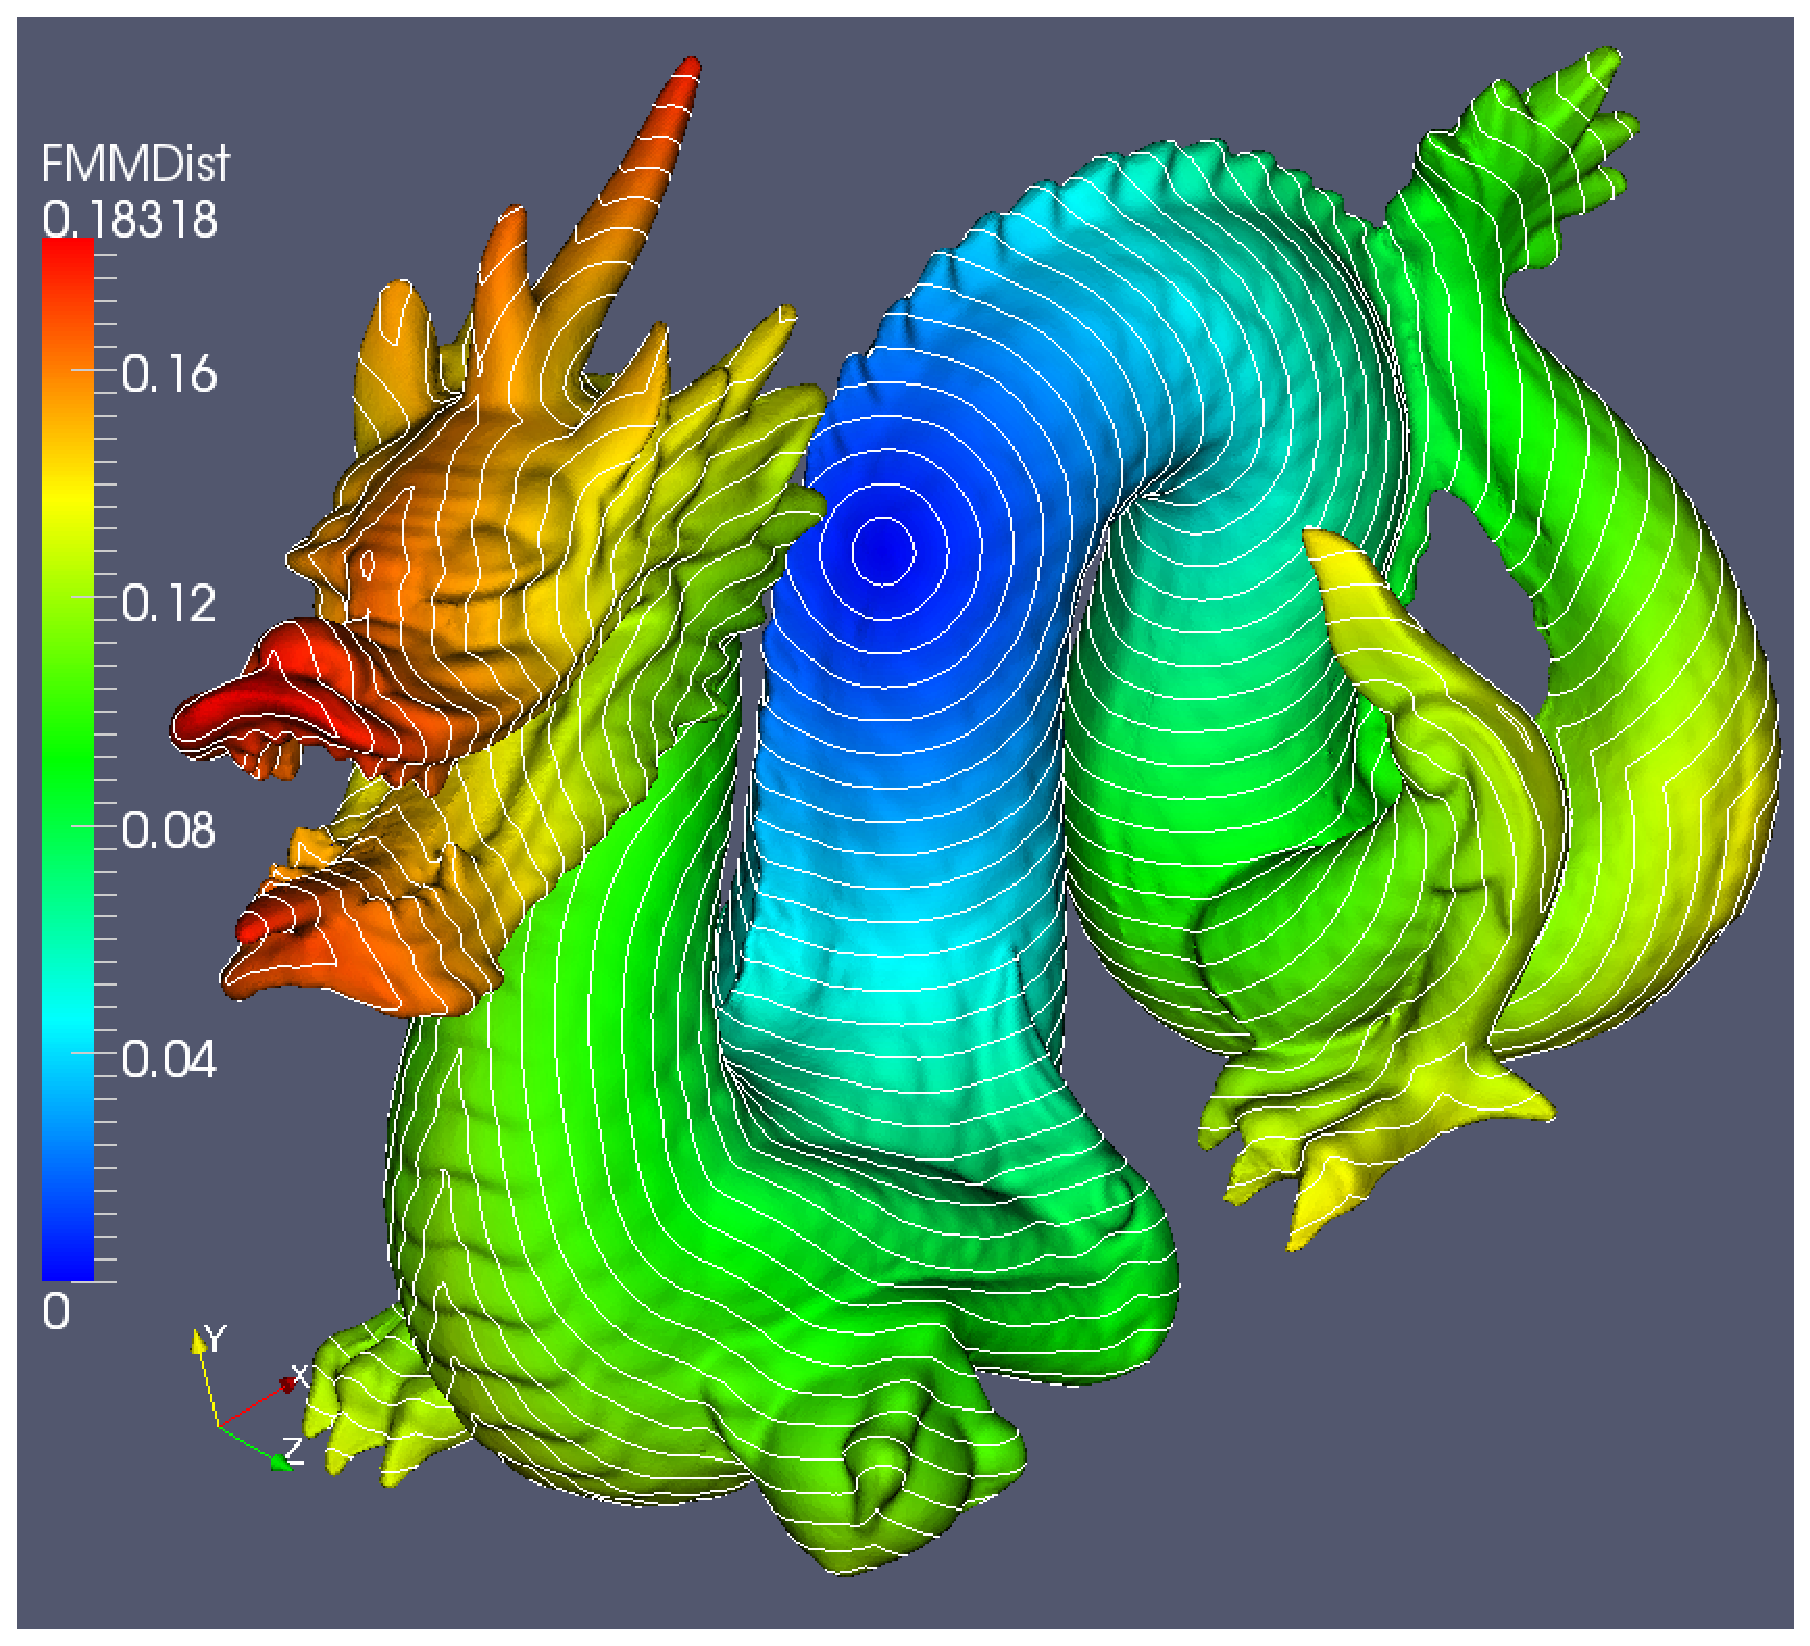
\includegraphics[width=\textwidth]{DragonGeodesic}
    \label{fig:DragonGeodesic}
  \end{subfigure}%
  ~ %add desired spacing between images, e. g. ~, \quad, \qquad etc.
    %(or a blank line to force the subfigure onto a new line)
  \begin{subfigure}[b]{0.45\textwidth}
    \centering
    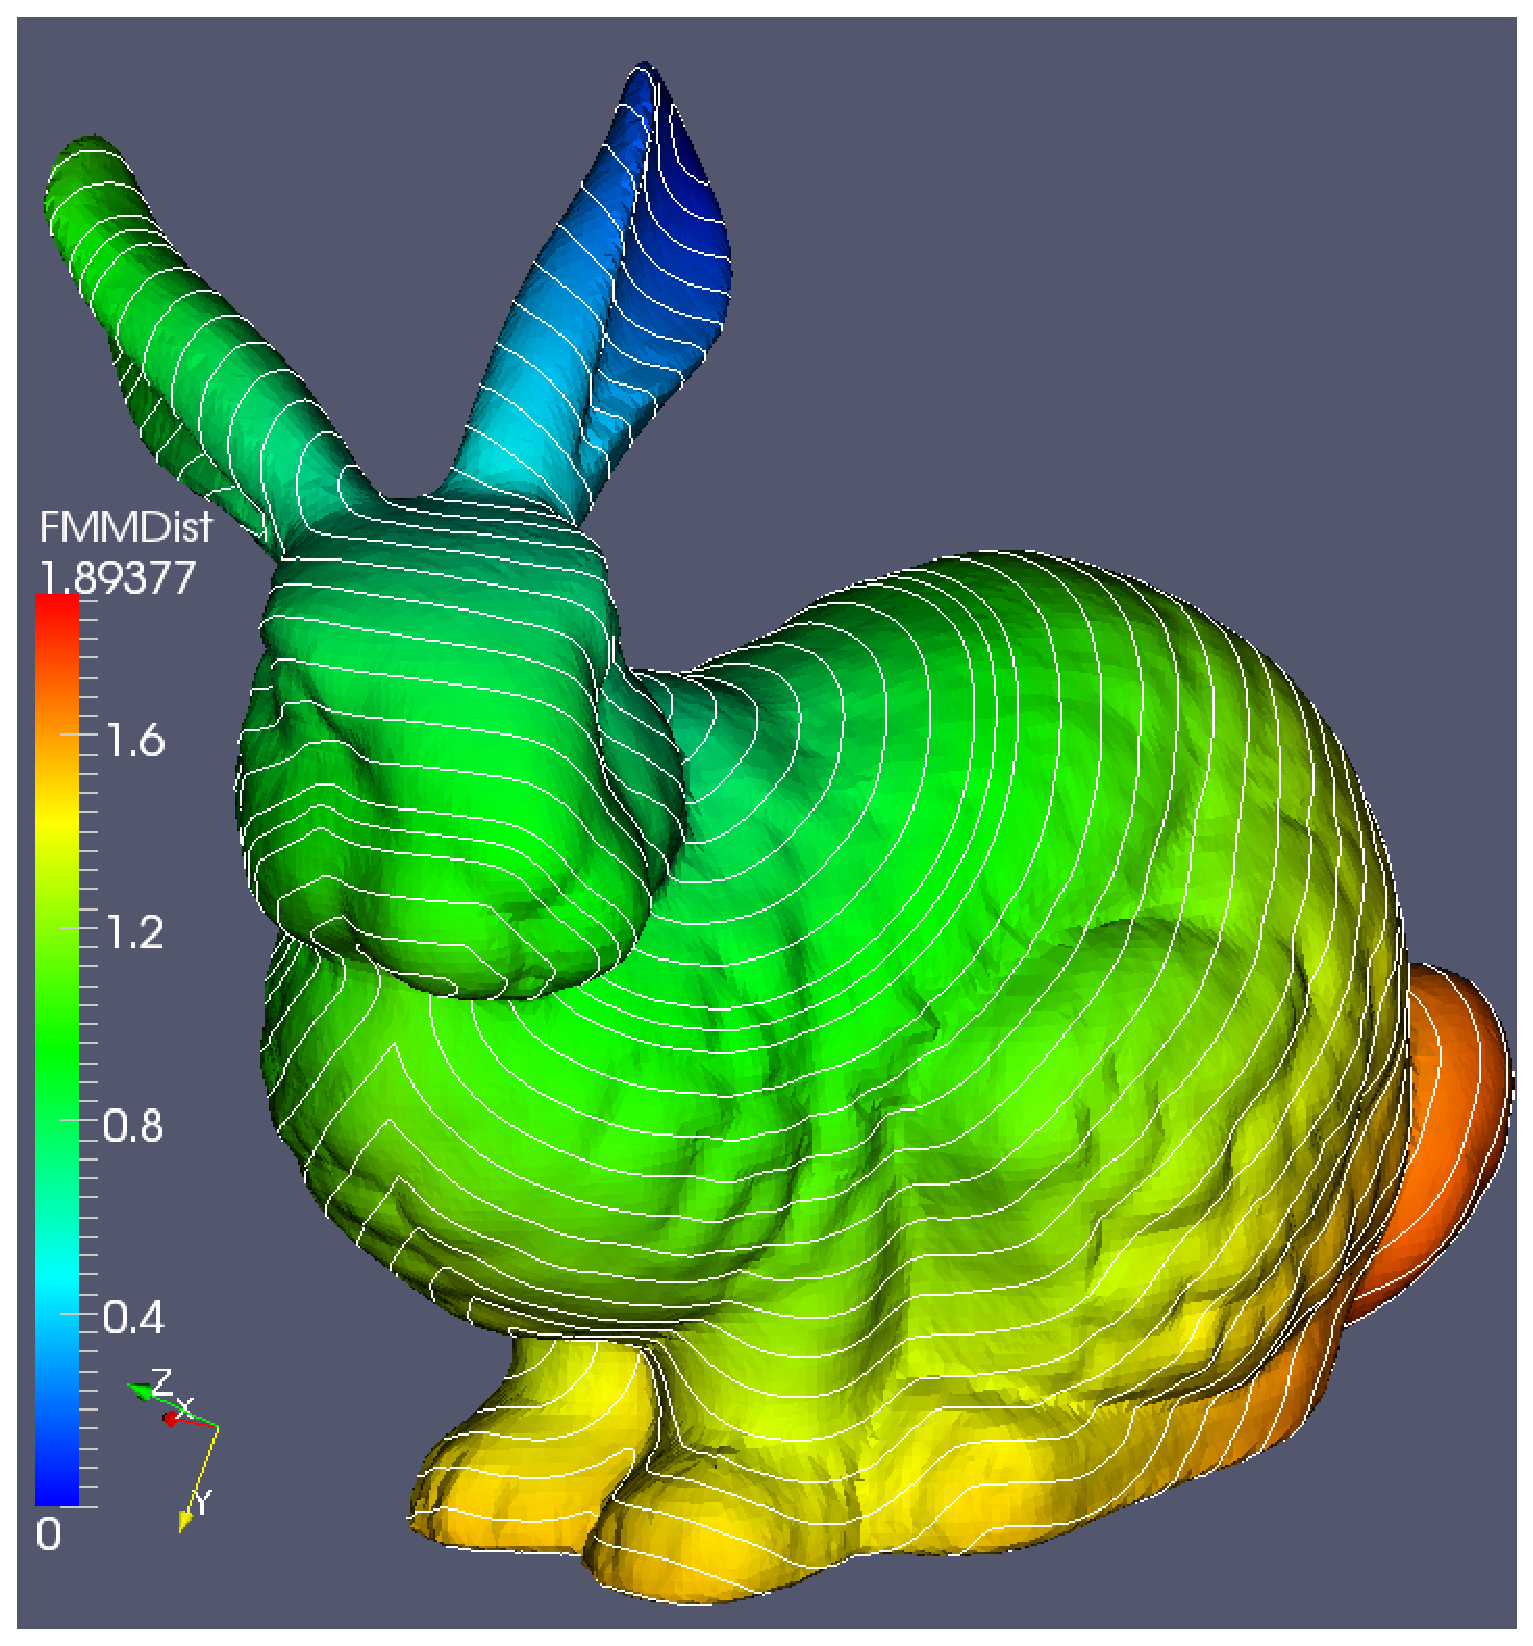
\includegraphics[width=\textwidth]{BunnyGeodesic}
    \label{fig:BunnyGeodesic}
  \end{subfigure}
\caption{Geodesic distance using fast marching.}
\label{fig:GeodesicDistances}
\end{figure}

The class \code{vtkPolygonalSurfaceContourLineInterpolator2} enables interactive tracing on polygonal surfaces. It is one of a growing family (see fig.~\ref{fig:GeodesicUMLs}(b))
of contour line interpolators that make the \vtk{vtkContourWidget} a powerful tool enabling contouring subject to a variety of constraints. 
It can replace \vtk{vtkPolygonalSurfaceContourLineInterpolator}, since it retains its public API but provides added functionality.

This interpolator is meant to be used in conjunction with a \vtk{vtkPolygonalSurfacePointPlacer} which constrains nodes dropped using a contour widget to vertices that lie on the surface of the mesh.
As points are interactively placed using the widget, it computes the path joining these nodes on the 2D manifold. There is a weak coupling between the classes allowing the picked point id to be queried by the interpolator from the placer, so that picking (which for large meshes can be expensive) may be performed only once.
The path may internally be generated using the Dijkstra algorithm, or by fast marching as described above. Fast marching with first order interpolation, unlike Dijkstra, allows the generation of smooth paths. Weighted constraints (as described above) may be used to preferentially displace the path based on features on the surface.

\subsection{Computation time}
The complexity of this method is $O(N log N)$, where $N$ is the number of mesh vertices. Hoppes et. al. compare, the runtime performance of this implementation with their and other implementations. The results are available in Table 1 ~\cite{Hoppes05}. On a mesh with ~10000 vertices, fast marching using this method is reported to take ~3.5s on a Pentium M 1.6GHz with 1GB RAM.


\section{Examples}

A subset of the scenarios discussed above are illustrated below with examples, included with this package. The Stanford Bunny (provided with this package) is used for all examples.

\subsection{Computing Geodesic distance}
The program \code{GeodesicDistanceExample.cxx} uses the \code{vtkFastMarchingGeodesicDistance} to compute a geodesic distance field on a surface.
Run it with the arguments

\begin{lstlisting}
  Bunny.vtp BunnyWithDistField.vtp
\end{lstlisting}

Pick any point on the displayed surface. The resulting image is the geodesic distance from the chosen point (see Fig.~\ref{fig:GeodesicDistances}) colored by the distance from the chosen point. The point data array \code{FMMDist} is populated with the distances.

\lstset{language=[ANSI]C++, floatplacement=!htb}
\begin{lstlisting}
  vtkFastMarchingGeodesicDistance *gd = vtkFastMarchingGeodesicDistance::New();
  gd->SetInputConnection(polydata);
  gd->SetFieldDataName("FMMDist");
\end{lstlisting}


\subsection{Specifying distance termination criteria}
\begin{figure}
  \centering
  \begin{subfigure}[b]{0.3\textwidth}
    \centering
    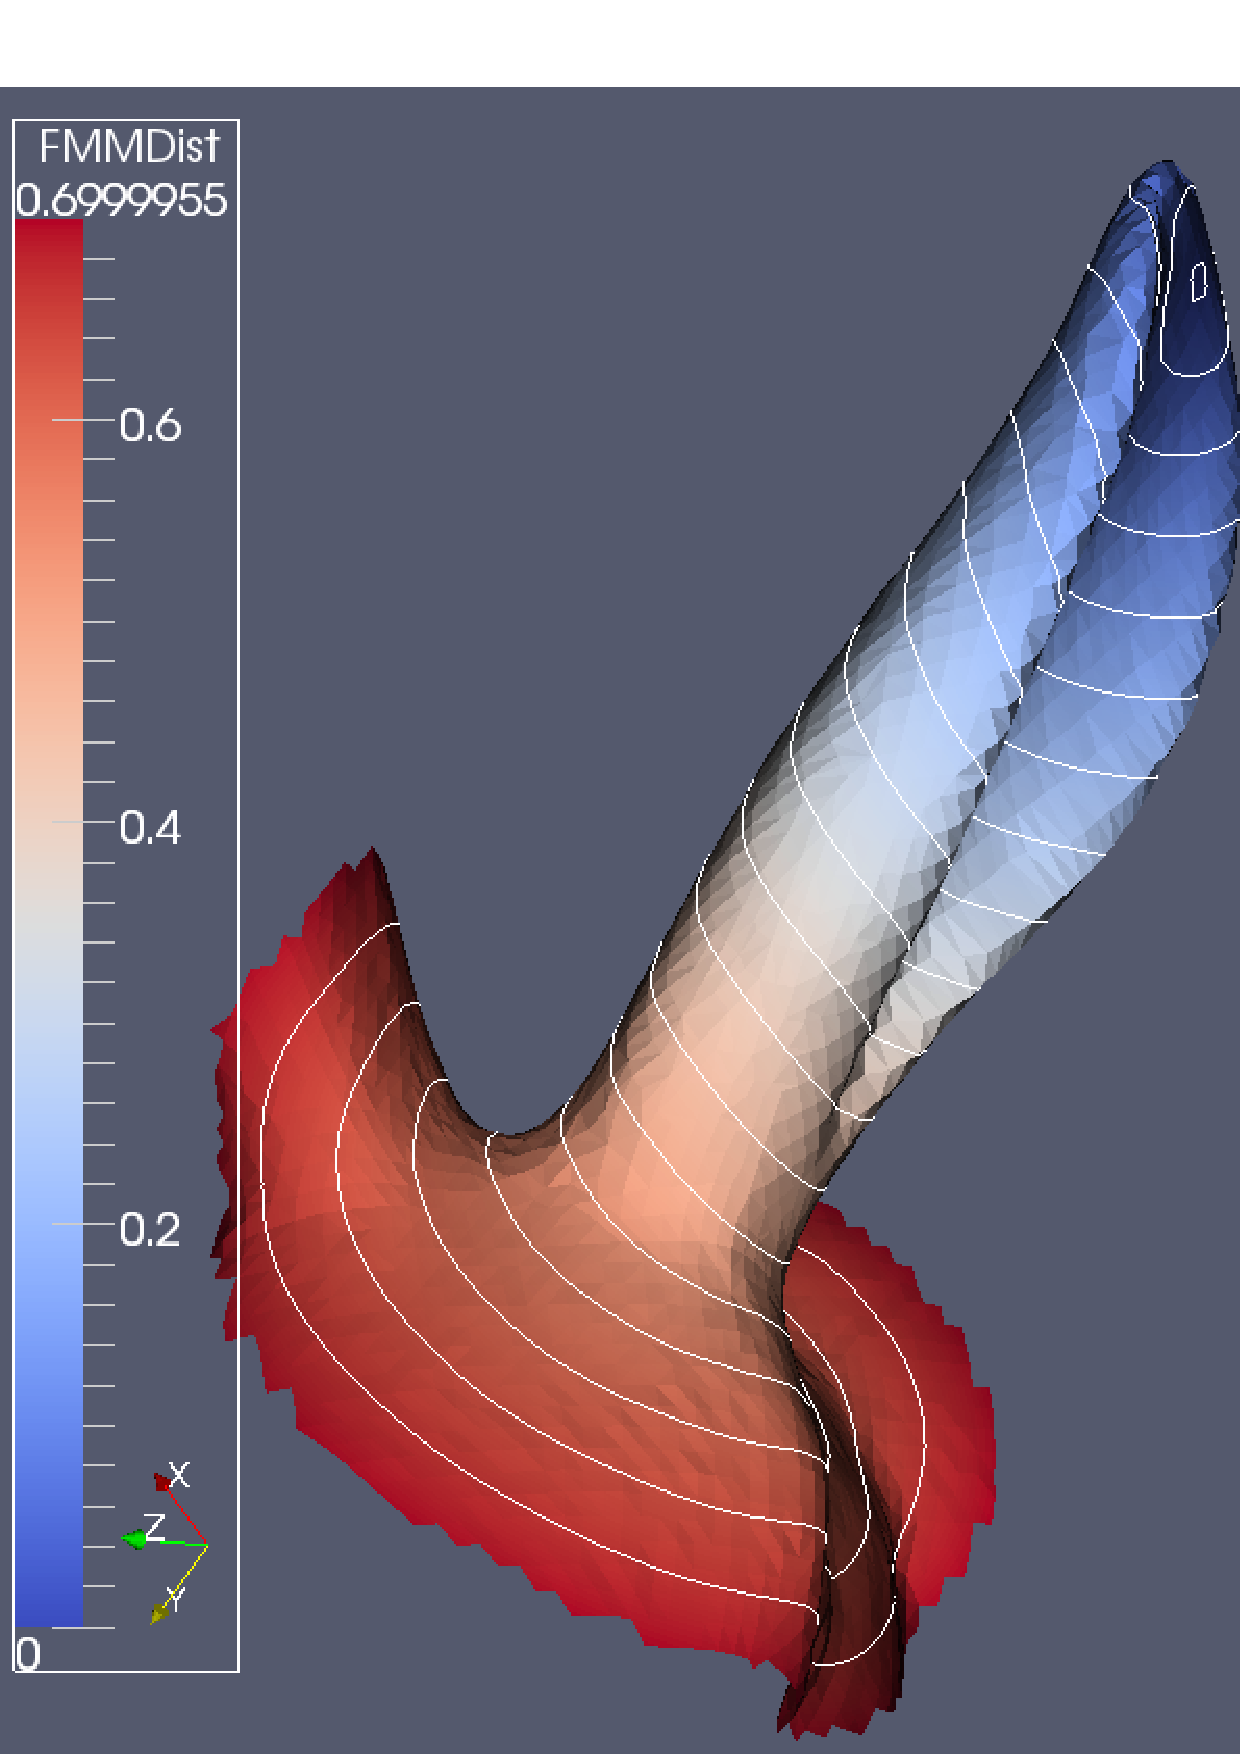
\includegraphics[width=\textwidth]{BunnyGeodesicDistanceStoppingCriteria}
    \label{fig:BunnyGeodesicDistanceStoppingCriteria}
    \caption{Fast marching upto a distance threshold of $0.7$ mm}
  \end{subfigure}
  \qquad
  \begin{subfigure}[b]{0.5\textwidth}
    \centering
    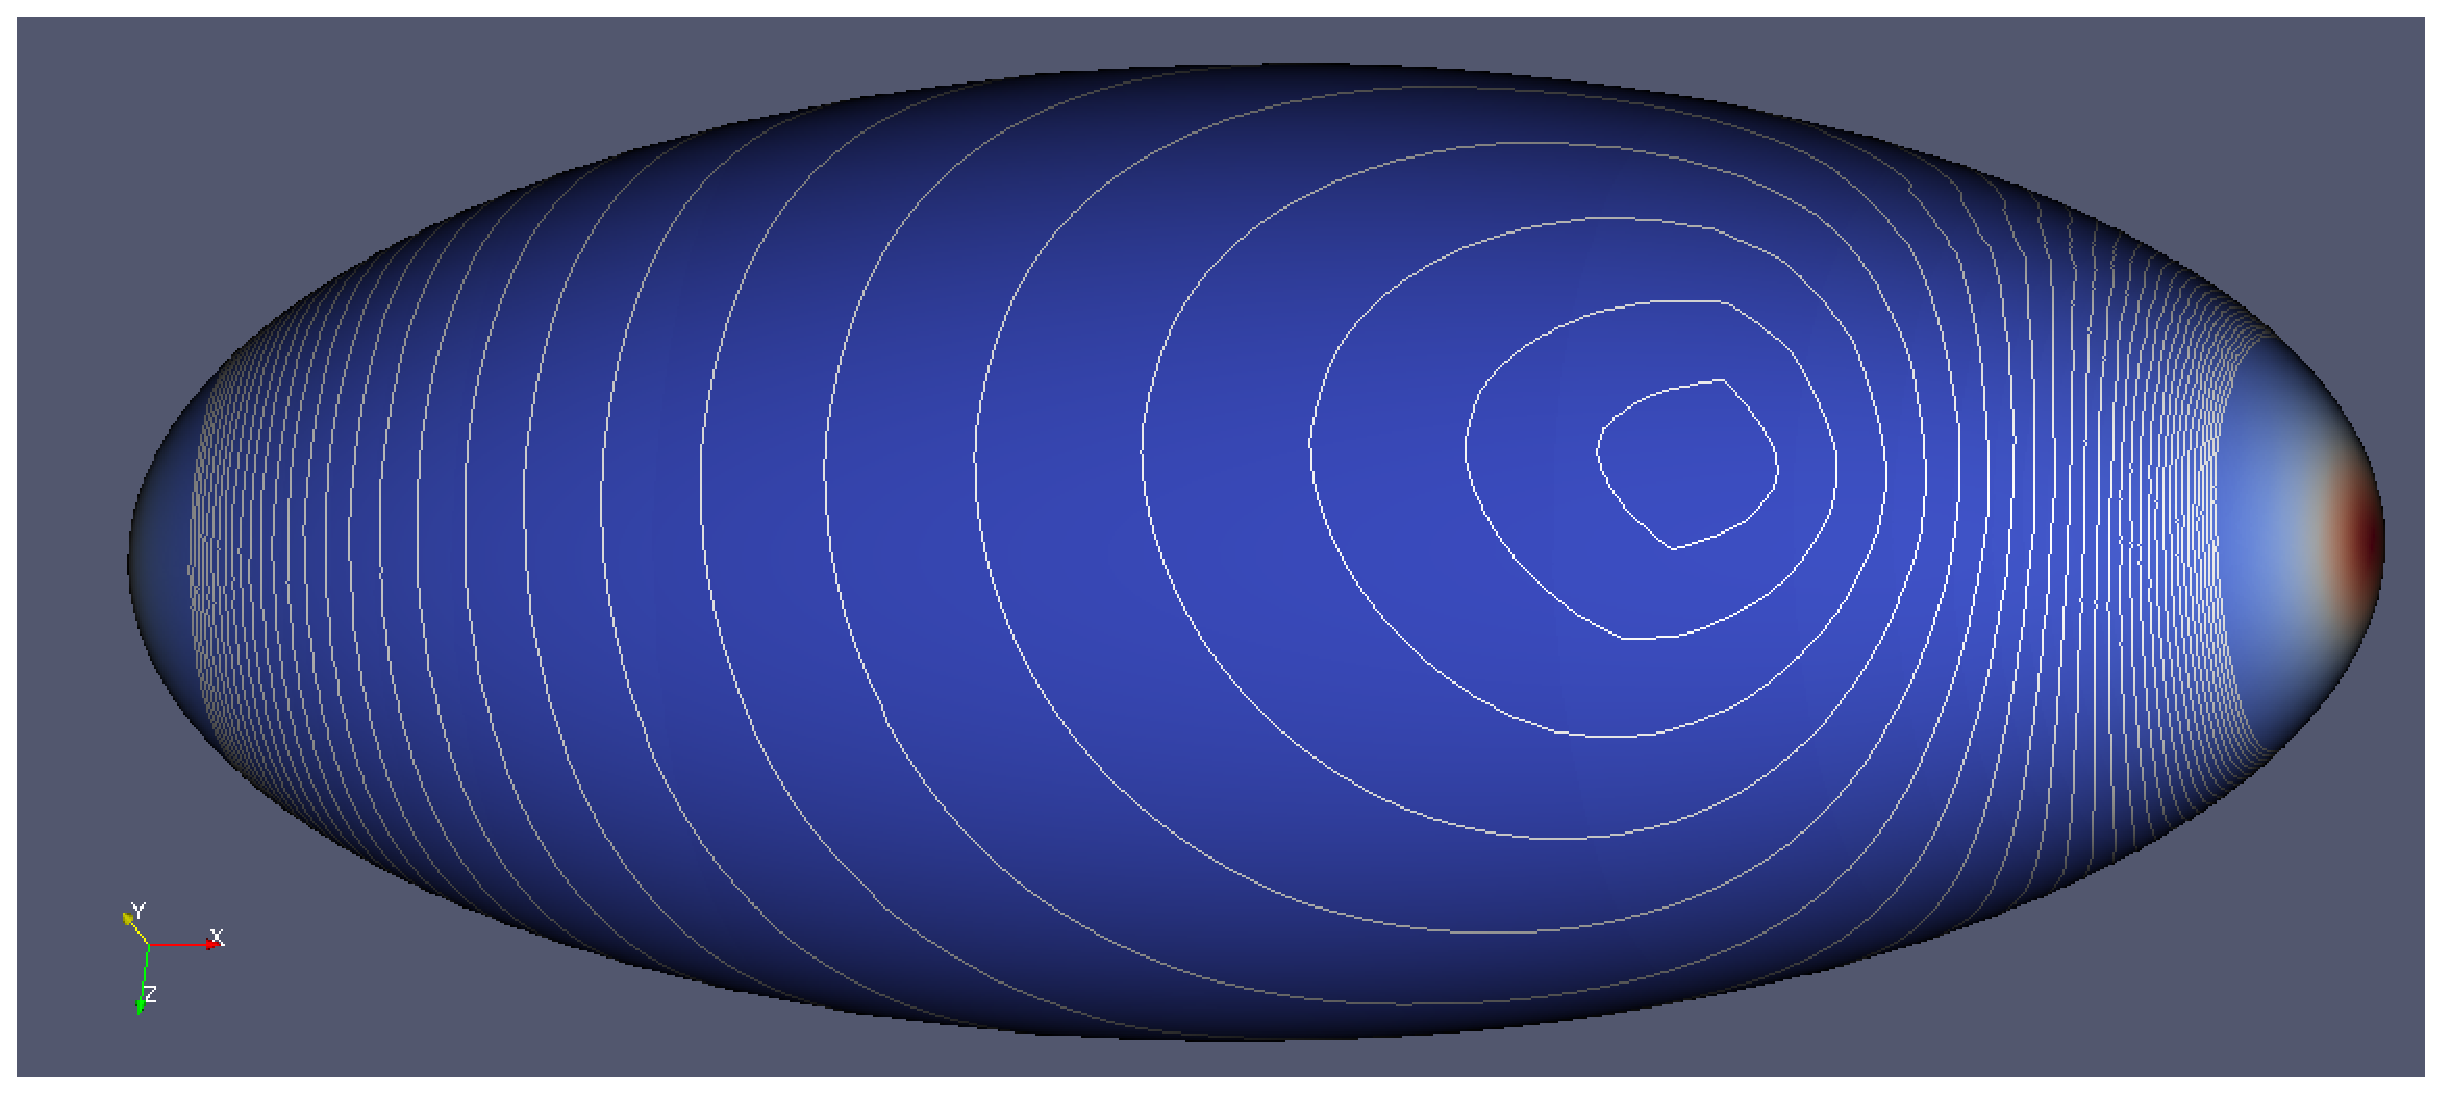
\includegraphics[width=\textwidth]{EllipsoidFastMarchingWithCurvatureGuidedPropagation}
    \label{fig:EllipsoidPropagationWt}
    \caption{Propagation weights are specified as the curvature of the point ids. This is observed in the assymetry in the isolines, which travel faster to the shorter axis of the point of least curvature on the ellipsoid.}
  \end{subfigure}
\caption{ }
\label{fig:GeodesicConstraints}
\end{figure}

Run the example as before but with the arguments
\begin{lstlisting}
  Bunny.vtp out.vtp --maxDist 0.7
\end{lstlisting}
This specifies distance threshold to terminate the front propagation by adding a line to the effect of
\begin{lstlisting}
  gd->SetDistanceStopCriterion(0.7);
\end{lstlisting}

The result is as shown in Fig.~\ref{fig:GeodesicConstraints}(a). The strategy can also be used to extract the surface within a given distance of the seed(s).

\subsection{Propagation Weights}
Propagation weights may be specified as a data array. For instance one can pass the mesh through the \vtk{vtkCurvatures} filter and specify the curvature data array as the propagation weight for the vertices.
\begin{lstlisting}
  gd->SetPropagationWeights(dataArray);
\end{lstlisting}
Run the same example with the arguments
\begin{lstlisting}
  Ellipsoid.vtp output.vtp --propagationWts CurvWt
\end{lstlisting}
This result is shown in Fig.~\ref{fig:GeodesicConstraints}(b).
Note that, as expected, the field traverses faster towards the left than towards the right.


\subsection{Exclusion Regions / Boundaries}
\begin{figure}
  \centering
  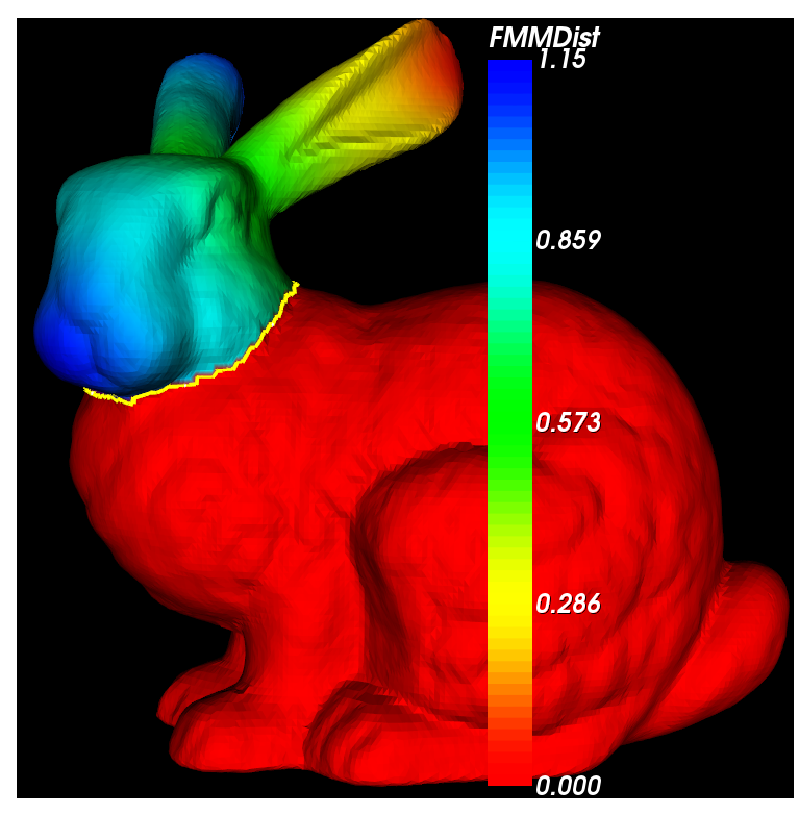
\includegraphics[width=0.45\textwidth]{BunnyGeodesicExclusionRegion}
  \caption{Exclusion regions or boundaries may be specified.}
  \label{fig:BunnyGeodesicExclusionRegion}
\end{figure}
Exclusion regions may be specified via a list of PointIds comprising the exclusion regions.
Note that if the exclusion regions, comprise a closed loop, around the seeds, this effectively becomes a boundary for the front. The following example demonstrates this. We run the same example with the arguments
\begin{lstlisting}
  Bunny.vtp output.vtp --exclusionContour
\end{lstlisting}
Once the render window comes up, drop points on the surface to trace a contour, looping back t to the first one, so as to close the contour.
After, the contour is closed, pick any point on the surface within the contour.
Here we extract the bunny's head (see Fig.~\ref{fig:BunnyGeodesicExclusionRegion} by tracing a contour around its neck and then pass these point ids as the exclusion region :
\begin{lstlisting}
  // Query the traced contour's point ids
  dijkstraContourInterp->GetContourPointIds(contourRepresentation, exclusionPtIds);
  gd->SetExclusionPointIds(ids); // Provide the ids as an exclusion region
\end{lstlisting}
You may peruse the example which also demonstates the use of a \vtk{vtkContourWidget} in conjunction with a \vtk{vtkDijkstraContourLineInterpolator} to trace the boundary contour.


\subsection{Tracing geodesic paths}
\begin{figure}
        \centering
        \begin{subfigure}[b]{0.3\textwidth}
                \centering
                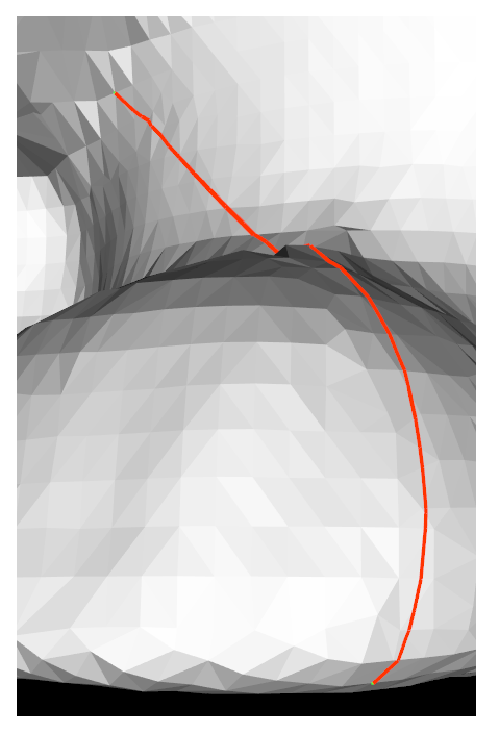
\includegraphics[width=\textwidth]{GeodesicPathFastMarchingFirstOrderInterp}
                \caption{Fast marching first order interpolation}
                \label{fig:GeodesicPathFMMFirstOrder}
        \end{subfigure}%
        ~ %add desired spacing between images, e. g. ~, \quad, \qquad etc.
          %(or a blank line to force the subfigure onto a new line)
        \begin{subfigure}[b]{0.3\textwidth}
                \centering
                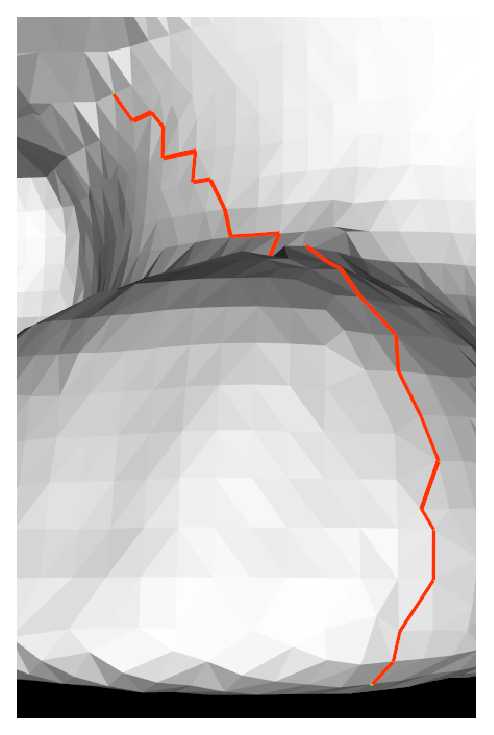
\includegraphics[width=\textwidth]{GeodesicPathFastMarchingZerothOrderInterp}
                \caption{Fast marching zeroth order interpolation}
                \label{fig:GeodesicPathFMMZerothOrder}
        \end{subfigure}
        ~ %add desired spacing between images, e. g. ~, \quad, \qquad etc.
          %(or a blank line to force the subfigure onto a new line)
        \begin{subfigure}[b]{0.3\textwidth}
                \centering
                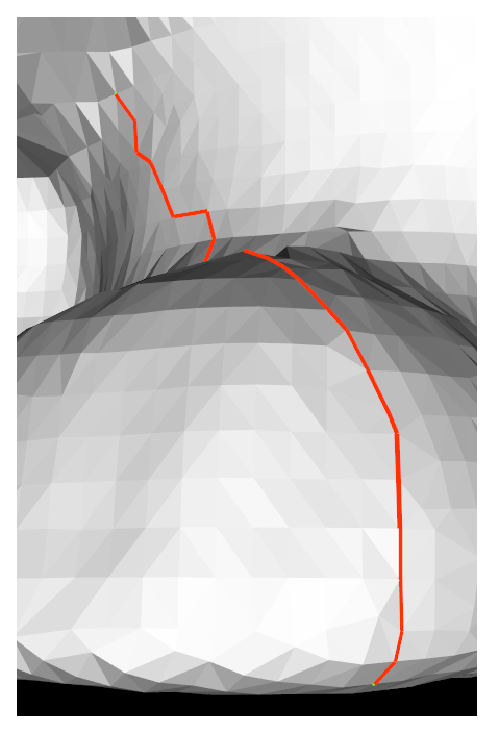
\includegraphics[width=\textwidth]{GeodesicPathDijkstraZerothOrderInterp}
                \caption{Dijkstra (zeroth order interpolation)}
                \label{fig:GeodesicPathDijkstra}
        \end{subfigure}
        \caption{Geodesic paths generated using various methods}
        \label{fig:GeodesicPaths}
\end{figure}
The program \code{GeodesicPathExample.cxx} demonstrates tracing a path interactively using a \vtk{vtkContourWidget} on a surface mesh. Its arguments are
\begin{lstlisting}
  surface.vtp [Method (0=Dijkstra,1=FastMarching)] [InterpOrder (0=NN,1=Linear)] [heightOffset]
\end{lstlisting}
Fig.~\ref{fig:GeodesicPaths} shows the paths generated using various methods.
Typically, the path computed using linear interpolation with fast marching is shorter than that computed with zeroth order interpolation using Dijkstra or with fast marching.
Note that the zeroth order paths using both methods (Dijkstra or FastMarching) need not be identical (as may also be observed in the figure). 
The Dijkstra method provides the true shortest zeroth order path, while that obtained from fast marching is (a) an approximation (b) clamps the first order path to its closest vertices and could be longer.
The computation times of both methods are nearly the same. The heightOffset argument allows one to displace the path in the direction of the surface normal.

\begin{lstlisting}
  vtkNew<vtkPolygonalSurfaceContourLineInterpolator2> interpolator;

  // Add all the surfaces to which the path is to be constrained
  interpolator->GetPolys()->AddItem( surfaceMesh );

  // Set the method to compute the geodesic (fast marching or dijkstra)
  interpolator->SetGeodesicMethodToFastMarching();
  interpolator->SetInterpolationOrder(1); // use first order interp
  rep->SetLineInterpolator(interpolator.GetPointer());

  // Setup the point placer used to constrain picking on the surface
  vtkNew<vtkPolygonalSurfacePointPlacer> pointPlacer;
  pointPlacer->AddProp(actor.GetPointer());
  pointPlacer->GetPolys()->AddItem( surfaceMesh );
  rep->SetPointPlacer(pointPlacer.GetPointer());

  // Snap the contour nodes to the closest vertices on the mesh
  pointPlacer->SnapToClosestPointOn();
\end{lstlisting}

%  Insert the bibliography using BibTeX

\bibliographystyle{plain}
\bibliography{references}
%
\end{document}

